\documentclass[a4paper,12pt]{article}
\usepackage[croatian]{babel}
\usepackage[utf8]{inputenc}
\usepackage{amsmath,amssymb}
\usepackage{graphicx}
\usepackage{xcolor}
\usepackage{tabularx}
\usepackage{lipsum}
\usepackage[useregional]{datetime2}
\usepackage{url}

\addtolength{\voffset}{-2cm} \addtolength{\textheight}{4cm}
\addtolength{\hoffset}{-1cm} \addtolength{\textwidth}{2cm}
\selectlanguage{croatian}

\newcommand*{\devname}{\texttt}
\newcommand*{\techspec}{\textsc}
\newcommand*{\term}{\textit}
\newcommand{\sitename}[1]{\texttt{"#1"}}
\renewcommand*{\emph}{\textbf}

\newcommand*{\maketitlepage}{%intro
  \begin{center}
    Sveučilište u Splitu\\
    Prirodoslovno-matematički fakultet\\
    Odjel za fiziku

    \bigskip
    \bigskip

    \large{Programski alati u fizici}


    \bigskip
    \bigskip

    \textbf{{\Large{Brojanje zvijezda na noćnom nebu}}}
  \end{center}
  \begin{center}
    \textbf{Frane Doljanin}\\
    \
  \end{center}
  \begin{center}
    Split, \DTMdate{2023-6-8}
  \end{center}
}

\begin{document}
\maketitlepage

\section*{Sažetak}
Cilj ovog rada bio je izračunati broj zvijezda na noćnom nebu koristeći podatke satelita Hipparcos. U radu je korištena javno dostupna baza podataka VizieR \cite{ct:VizieR} s podatcima o zvijezdama, a koji su obrađeni u programskom jeziku Python. U radu je opisan postupak obrade podataka i prikazani su rezultati sa zaključkom - u prosjeku se vidi \mbox{$\approx$ 4200} zvijezda na noćnom nebu.

\section{Uvod}
Fascinacija noćnim nebom često je zanemarena u gradovima kao posljedica onečišćene atmosfere i svjetlosnog zagađenja. Ovaj program omogućuje izračun broja zvijezda na noćnom nebu, te ovisnost istog o promjeni lokacije promatrača.
\par
U ovom radu korišteni su podatci satelita Hipparcos, koji je u razdoblju od 1989. do 1993. godine snimio preko 100 000 zvijezda. Podatci su javno dostupni na stranici \mbox{VizieR} \cite{ct:VizieR}, a katalog kojim se koristimo naziva je \devname{I/239/hip\_main}.

Naravno, svih 100 000 zvijezda nije vidljivo na nebu, već samo one najsjajnije, pozicionirane tako da ih Zemlja ne prekriva. Da bismo filtrirali samo takve zvijezde, koristimo se stupcima \techspec{RAdeg}, \techspec{DEdeg} i \techspec{VMag}.

\subsection{Položaj na nebeskoj sferi}
Položaj zvijezde na noćnom nebu ovisi o položaju promatrača na Zemlji, stoga je potreban način koji bi trajno opisao poziciju zvijezde neovisno o promatraču. Zato se koristimo rektascenzijom i deklinacijom. \cite{ct:equatorial_coords}

\emph{Rektascenzija} (eng. \term{right ascension}, pokrata \techspec{RA}) je koordinata koja mjeri kut između ravnine nebeskog meridijana i ravnine satne kružnice zvijezde. Ova koordinata određuje položaj zvijezde u smjeru istoka. Rektascenzija je ekvivalentna pojmu geografske dužine na Zemlji, gdje 360 stupnjeva predstavlja puni krug od 24 sata.

\emph{Deklinacija} (eng. \term{declination}, pokrata \techspec{DE}), s druge strane, izražava se u stupnjevima i mjeri kut između nebeskog ekvatora i zvijezde. Ova koordinata određuje položaj zvijezde u smjeru sjevera ili juga, ovisno o tome je li deklinacija pozitivna ili negativna. Deklinacija se mjeri u rasponu od -90° do +90°.

Kombinacija rektascenzije i deklinacije omogućuje jedinstveno određivanje položaja zvijezda na nebeskoj sferi. Ove koordinate omogućuju precizno lociranje zvijezda bez obzira na promatračevu lokaciju na Zemlji.

U ovom radu, koristimo stupce \techspec{RAdeg} (rektascenzija u stupnjevima) i \techspec{DEdeg} (deklinacija u stupnjevima) iz podataka satelita Hipparcos kako bismo odredili položaj zvijezda na noćnom nebu. Prikaz ovih koordinata možemo vidjeti na slici \ref{fig:ra_de}.

\begin{figure}[h]
  \begin{minipage}[t]{0.40\linewidth}
    \centering
    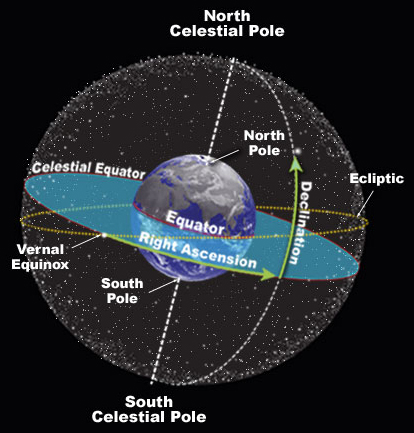
\includegraphics[height=150px]{assets/ext-ra_de.jpg}
    \caption{Prikaz nebeskih koordinata - rektascenzija i deklinacija. \cite{ct:ra_de-img}}\label{fig:ra_de}
  \end{minipage}
  \begin{minipage}[t]{0.55\linewidth}
    \centering
    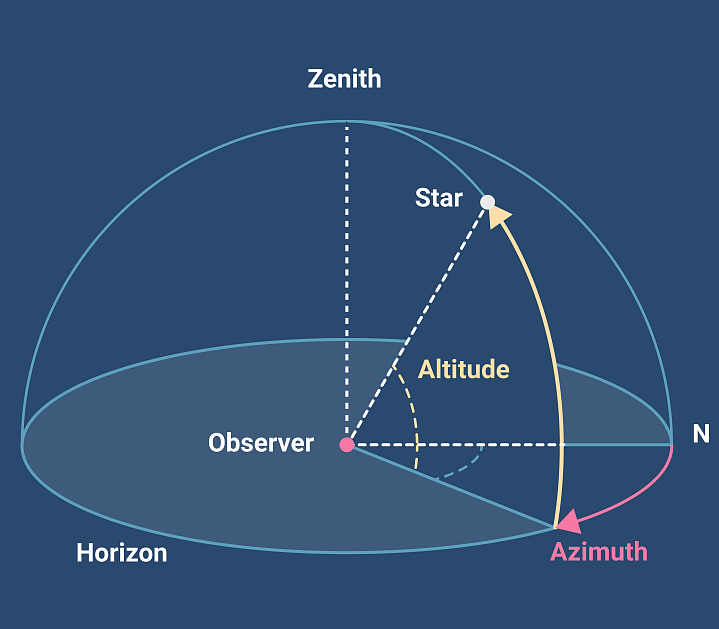
\includegraphics[height=150px]{assets/ext_el-as.png}
    \caption{Elevacija i azimut. \cite{ct:el_as-img}}\label{fig:el_as}
  \end{minipage}
\end{figure}

\subsection{Položaj na noćnom nebu}
Kada je riječ o trenutnom položaju zvijezde na nebu iz perspektive promatrača, koristimo se azimutom i elevacijom.

\emph{Azimut} je kut između vertikalne ravnine koja prolazi nebeskim polom do vertikalne ravnine koja prolazi točkom opažanja. Mjeri u rasponu od 0° do 360°, gdje 0° predstavlja sjever, 90° istok, 180° jug i 270° zapad.

\emph{Elevacija} je kut između horizontalne ravnine i linije koja spaja promatrača i zvijezdu. Mjeri se u stupnjevima i ima raspon od -90° do +90°. Kada je elevacija pozitivna, zvijezda je iznad horizonta i promatrač ju može vidjeti. Ako je elevacija negativna, zvijezda je ispod horizonta i nije vidljiva s promatračevog položaja.
Prikaz elevacije i azimuta možemo vidjeti na slici \ref{fig:el_as}, gdje \term{Altitude} predstavlja elevaciju.

Dakle, potrebno je, poznavajući trenutno vrijeme i promatračeve geografske koordinate, izračunati azimut i elevaciju za svaku zvijezdu. U slučaju da je elevacija pozitivna, zvijezdu je moguće vidjeti po pitanju pozicije, a u slučaju da je negativna, nalazi se ispod horizonta i sigurno nije vidljiva.

\subsection{Sjaj zvijezde}
Još je potrebno odrediti može li ljudsko oko u idealnim noćnim uvjetima vidjeti zvijezdu. To ovisi o prividnoj magnitudi \cite{ct:vmag}, koja mjeri prividni sjaj zvijezde na nebu, normaliziran na vrijednost koju bi imao izvan atmosfere. Ovisi o samoj zvijezdi i udaljenosti od Zemlje.

Prividna magnituda se mjeri na skali u kojoj manje vrijednosti označavaju sjajnije objekte, dok veće vrijednosti označavaju tamnije objekte. Na primjer, vrlo svijetle zvijezde imaju negativne vrijednosti prividne magnitude, dok tamnije zvijezde imaju pozitivne vrijednosti. Prosječno ljudsko oko vidi zvijezde do magnitude 6.5, pa zanemarujemo sve one zvijzde s magnitudom većom od navedene.


\section{Diskusija i rezultati}
Podatci su obrađeni u programskom jeziku Python.

\subsection{Postavljanje}
Prije svega, potrebno je preuzeti bazu podataka na lokalno računalo. Datoteka s podatcima zauzima $\approx$ 50MB i zbog svoje veličine nije uključena u remote.
Da bi datoteka bila preuzeta, pokreće se skripta \devname{fetcher.py}. Ona koristi libraryje \devname{requests} za preuzimanje datoteke s interneta, \devname{zlib} za dekompresiju s obzirom na to da je datoteka \term{gzipirana}, te \devname{os} za pisanje na disk. Nakon što funkcija \devname{download\_and\_save} završi s preuzimanjem, datoteka \devname{I\_239\_hip\_main.dat} i dalje nije pogodna za obradu jer se podatci nalaze u formatu koji je podržan samo od strane \devname{Astropy} paketa, a i prevelika je za učitavanje u memoriju ako ćemo je više puta pokretati. Kako bi se izbjegle poteškoće, funkcija \devname{data\_to\_csv} pretvara datoteku u CSV format pogodan za obradu, i to samo one stupce koji su nam potrebni - \techspec{VMag}, \techspec{RAdeg}, \techspec{DEdeg}.

\subsection{Brojač}
Nakon uspješnog postavljanja, možemo početi s brojanjem.
Kako broj vidljivih zvijezda ovisi o poziciji na Zemlji, korisnik je upitan za promatrani grad, pa preko Geocoding API-ja dobivamo geografske koordinate grada. Trenutno UTC vrijeme doznaje se pomoću \devname{datetime} libraryja.
Sada u CSV datoteci idemo liniju po liniju, pritom učitavajući samo trenutnu zvijezdu u memoriju. Svaku zvijezdu proslijedimo funkciji \devname{check\_is\_visible}, koja vraća \devname{True} ako je zvijezda vidljiva, a \devname{False} ako nije. Ako je zvijezda vidljiva, povećamo brojač vidljivih zvijezda za 1. Na kraju, ispišemo broj vidljivih zvijezda.

Funkcija \devname{check\_is\_visible} provjerava prethodno navedene fizikalne uvjete, odnosno činjenicu da \techspec{VMag} mora biti manja od 6.5 i da je elevacija pozitivna. Sama implementacija jasna je iz koda. Za transformaciju iz \techspec{RAdeg} i \techspec{DEdeg} u azimut i elevaciju koristio sam se formulama s interneta. \cite{ct:transform} 

\begin{figure}[h]
  \begin{minipage}[t]{0.48\linewidth}
    \centering
    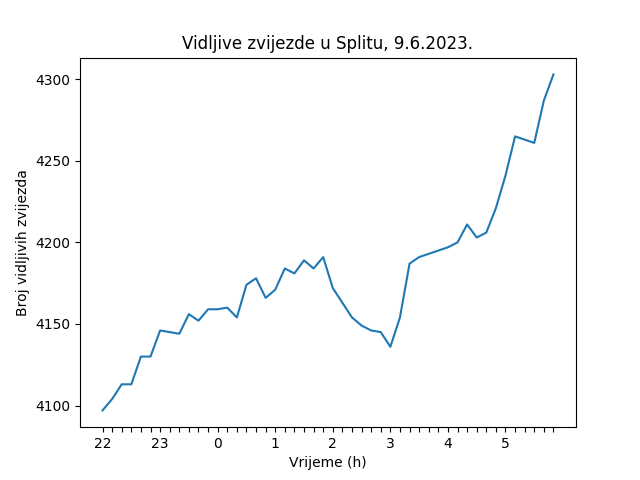
\includegraphics[height=150px]{assets/plt-stars_night.png}
    \caption{Broj zvijezda godišnje}\label{fig:stars_night}
  \end{minipage}
  \begin{minipage}[t]{0.48\linewidth}
    \centering
    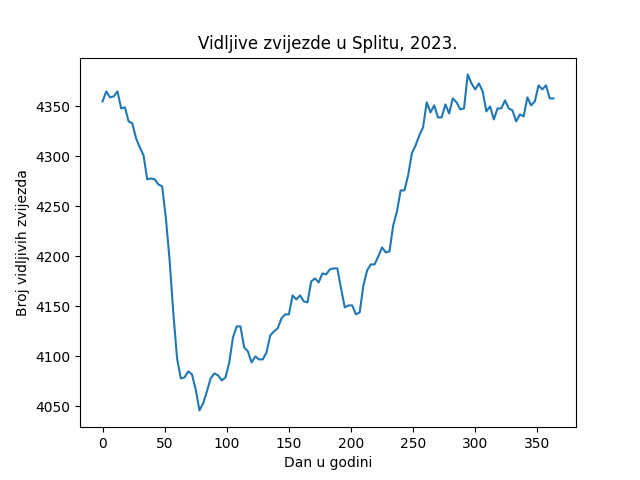
\includegraphics[height=150px]{assets/plt-stars_year.png}
    \caption{Broj zvijezda ponoći}\label{fig:stars_year}
  \end{minipage}
\end{figure}

Na slici \ref{fig:stars_night} prikazan je broj vidljivih zvijezda po satu noći u Splitu od 22 do 06 sati. Prosječan broj iznosi 4178. Na slici \ref{fig:stars_year} prikazan je broj vidljivih zvijezda po danu godine 2023. godine u Splitu u 00:00 sati po UTC vremenu. Prosječan broj iznosi 4235. Iako varijacija nije značajna, ipak postoji i konzistentna je.

\section{Zaključak}
Iz rezultata programa jasno je da broj zvijezda značajno ne varira tijekom noći i godine te da je svjetlosno onečišćenje krivac za slabu vidljivost zvijezda tijekom noći, budući da bi, sudeći po brojkama, u idealnim uvjetima trebao biti spektakl.

Kôd je mogao izbaciti točniji rezultat tako što u obzir uzme reljef, zgrade i sl. te uračuna onečišćenje, ali to je izvan okvira ovog rada. Također, mogao se značajno brže izvršavati da je napisan u C++ ili nekom drugom kompajliranom jeziku koji podržava višedretvenost (eng. \term{multithreading}). Međutim, uzimajući u obzir namjenu programa i očekivanu količinu izvršenja, vrijeme izvršavanja od najviše dvije sekunde je prihvatljivo.


\begin{thebibliography}{9}
  \bibitem{ct:VizieR}
    VizieR Online Data Catalog: I/239 (Hipparcos, 1997),\\
    \url{http://cdsarc.u-strasbg.fr/viz-bin/nph-Cat/txt.gz?I/239/hip\_main.dat}
  \bibitem{ct:equatorial_coords}
    Nebeski ekvatorski koordinatni sustav, \sitename{Wikipedia} \\
    \url{https://en.wikipedia.org/wiki/Equatorial_coordinate_system}
  \bibitem{ct:vmag}
    Prividna magnituda, \sitename{Planetary Sciences}\\
    \url{https://planetary-science.org/astronomy/magnitudes-brightness/}
  \bibitem{ct:transform}
    Tansformacija iz \techspec{RAdeg} i \techspec{DEdeg} u azimut i elevaciju, \sitename{Astrogreg}\\
    \url{https://astrogreg.com/convert_ra_dec_to_alt_az.html}
  \bibitem{ct:ra_de-img}
    Slika nebeskih koordinata, \sitename{SDSS Voyages}\\
    \url{https://voyages.sdss.org/preflight/locating-objects/ra-dec/}
  \bibitem{ct:el_as-img}
    Slika elevacije i azimuta, \sitename{timeanddate}\\
    \url{https://c.tadst.com/gfx/1200x630/horizontal-coordinate-system.png}

\end{thebibliography}

\end{document}


%%%%%%%%%%%%%%%%%%%%%%%%%%%%%%%%%%%%%%%%
%    Izmijenjeno od:       Uzorak dokumenta za seminar iz moderne fizike, 2019.          %
%                            Mislav Cvitković, Split, svibanj 2019.                          %
%%%%%%%%%%%%%%%%%%%%%%%%%%%%%%%%%%%%%%%%